\documentclass{article} % For LaTeX2e
\usepackage{nips15submit_e,times}
\usepackage{hyperref}
\usepackage{url}
\usepackage{graphicx}
%\documentstyle[nips14submit_09,times,art10]{article} % For LaTeX 2.09


\title{DSGD for MF on Spark 10605 15 Fall}


\author{
Jingyuan Liu\\
AndrewId: jingyual\\
\texttt{jingyual@andrew.cmu.edu} \\
}


\newcommand{\fix}{\marginpar{FIX}}
\newcommand{\new}{\marginpar{NEW}}


\nipsfinalcopy % Uncomment for camera-ready version


\begin{document}
\maketitle



\section{Question 1}


While both algorithms could achieve the goal of Matrix Factorization, we
realized that DSGD is much more scalable than SVD. With DSGD, we could generate
stratum with several independent blocks. The computation of each block is
independent, which makes the algorithm very scalable to run on several cores or
machines in an elegant parallel way.



\section{Question 2}


\subsection{Question2.1}
Matrix Factorization could be seen as a kind of ``topic model''. Basically, we
could see that the factor number is the chosen topic number. For the W matrix,
we could see it as the importance of doc over topics. For the H matrix, we could
see it as the importance of topic over words.


\subsection{Question2.2}
As we mentioned above, the H matrix could be explained as the importance of
topic over words. Therefore, if we want to find the top k words in a topic, we
could use the H matrix to do it. We could set the ith row of a H matrix, and then find
the top k words in the ith row. These top k words is the top k words of topic i.



\section{Question 3}
I think holding on all other conditions, the Spark implementation should be
faster than the Hadoop implementation.

First of all, Spark is lazy evaluation, which uses the DAG and wait to execute
after accumulating series of transformations.

Besides, the MapReduce framework is not suitable for DSGD-MF. Bascially, we know
that MapReduce is based on stream and sort, which is not suitable for this
iterative steps.



\section{Question 4}


\subsection{Question 4.1}
The trend is:
\begin{figure}[h]
\begin{center}
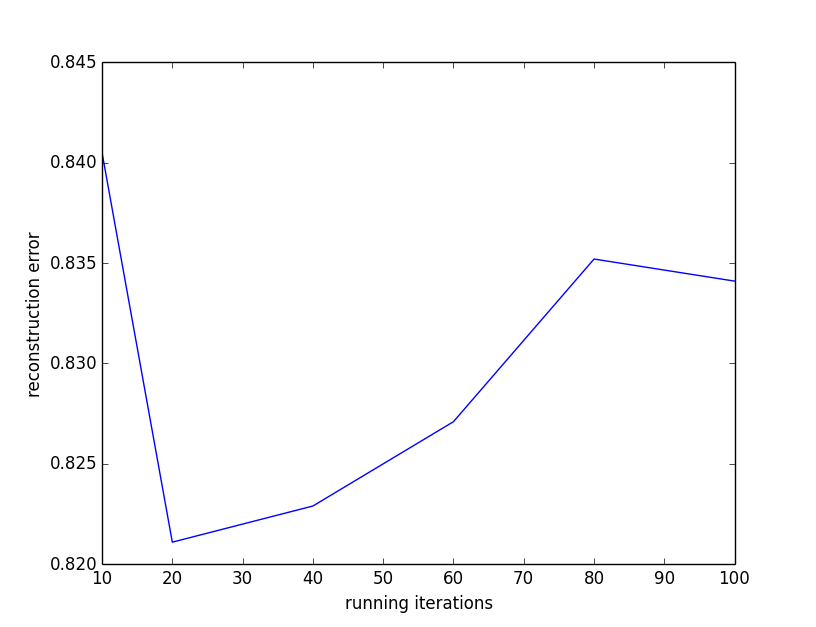
\includegraphics[width=10cm]{pic/q41.png}
\end{center}
\caption{Error over iteration}
\end{figure}

We could see at first, with the increase of iterations, the reconstruction error
would decrease. Then it would slowly increase with more iterations.


\subsection{Question 4.2}
The trend is:
\begin{figure}[h]
\begin{center}
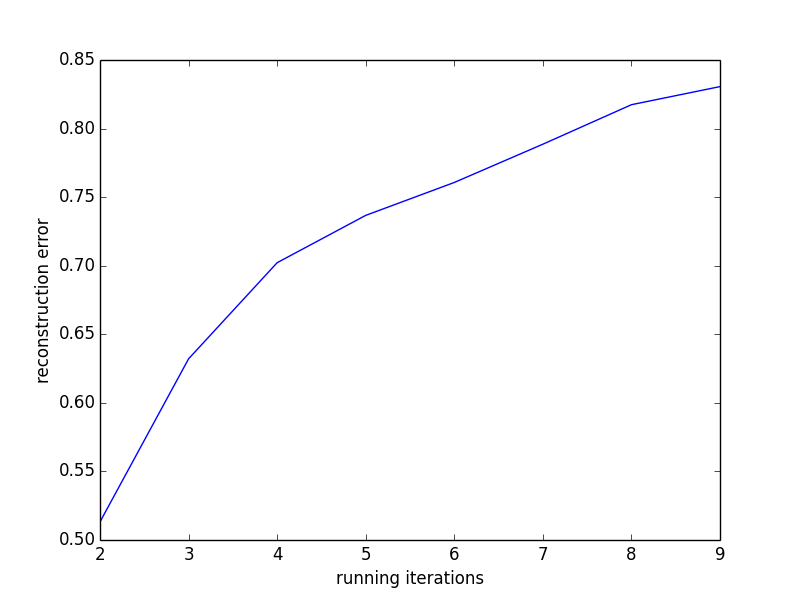
\includegraphics[width=10cm]{pic/q42.png}
\end{center}
\caption{Error over worker}
\end{figure}

We could see that as the increase of workers, the error would increase. This is
quite reasonable because with increase of workers, the error of approximation
like number of iterations would be more influential.

\subsection{Question 4.3}
The trend is:
\begin{figure}[h]
\begin{center}
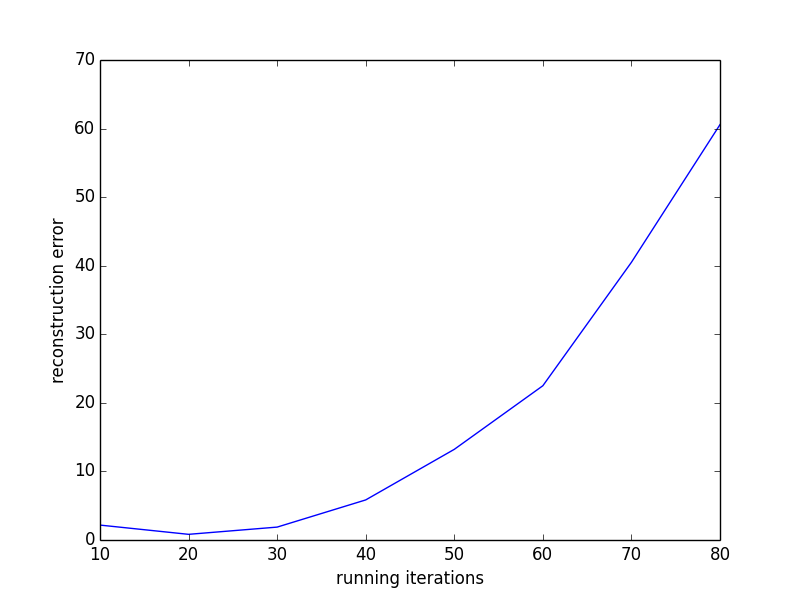
\includegraphics[width=10cm]{pic/q43.png}
\end{center}
\caption{Error over factors}
\end{figure}

We could see at first, with the increase of topics or factors, the error would
decrease. Then with the increase of factors after 20, the error would increase
very fast. This is because we set too many topics to the dataset.

\subsection{Question 4.4}
The trend is:
\begin{figure}[h]
\begin{center}
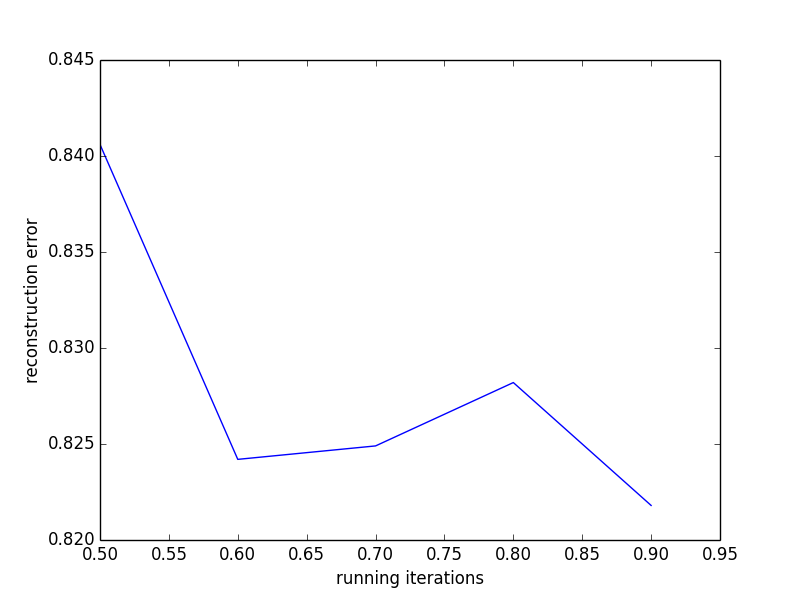
\includegraphics[width=10cm]{pic/q44.png}
\end{center}
\caption{Error over beta}
\end{figure}

We could see the trend is at first decrease, and then is stable, not sensitive
to the increase of beta



\section{Question 5}

I received helps from Chenran Li, whose AndrewId is chenranl. He told me how to
design the blockify matrix function and how to understand the perform sgd
function.


\end{document}
